\documentclass[twocolumn, 9pt]{jsproceedings}

\interfootnotelinepenalty=10000

\title{Monocular Estimation of Spatial Displacement}

\author{Helio Perroni Filho (Doctorate Course, 1st year)\authorrefmark{1}}

\affiliation{Intelligent Robotics Laboratory, OHYA's group}

\abstract{
This article investigates how cues in monocular vision can be explored to estimate a robot's position relative to a set of visible landmarks. It presents a model for reasoning about the problem, a data set recorded to test the model, provisional solutions for the problems of selecting and comparing landmarks on images, and a set of statistical results computed from those elements. The results point towards the feasibility of visual estimation of landmark-relative displacement from monocular images.
}

\keywords{Image Processing, Machine Learning, Sensing}

\begin{document}
\thispagestyle{myheadings}
\markright{2013年度 第3回 山彦シンポジウム [2014/2/17--2/19 国立オリンピック記念青少年総合センター]}
\maketitle

\authorreftext{1}{Graduate School of Systems and Information Engineering,\\ University of Tsukuba}

\section{Introduction}

Landmark-based navigation methods have become a central topic of research in mobile robotics. This is because, in contrast to intrinsic localization methods such as odometry, localization relative to reliable external references does not suffer from an unrecoverable accumulation of drift errors. However it is not without its own open questions, such as how landmarks should be selected, how can they be identified, and how the robot's position relative to them can be computed. This last problem is specially difficult for monocular vision systems, where depth information is not immediately available. On the other hand, given the current ubiquity of simple monocular cameras, the development of effective navigation methods on them could open the doors for a range of new applications.

This article investigates how cues in monocular vision can be explored to estimate a robot's position relative to a set of visible landmarks. It starts by constructing a model for reasoning about variations in the perception of objects due to physical displacements. An hypothesis is made that it is possible to estimate physical displacements from measurements of such variations. A data set is required to test this hypothesis, so a procedure for recording one is described, and its resulting characteristics are reported. Next the practical problem of how to identify and relate landmarks in the images of the data set is approached, and a provisional solution is devised. Statistics on the data set are calculated and analyzed in view of the proposed displacement model, and shown to be in agreement with the model's predictions overall. The article concludes with a discussion on future applications of the model, in particular how a displacement estimation system could be implemented based on it.

\section{Displacement Estimation Model}

Consider a robot equipped with a single front-mounted camera, wandering about an environment populated by stationary objects (or {\it landmarks}) by alternating among three {\it modes} of movement: straight (forward / backward), turning (clockwise / counter-clockwise) and sideways (left / right). As the robot's position changes relative to landmarks in its field of view, their images change in predictable ways:

\begin{itemize}
\item When the robot moves forward in a straight line, landmarks tend to appear bigger as they draw closer, and to drift towards the borders of the image as they are passed by (see Figure~\ref{fig:mode_straight});
\item When the robot turns in place, landmarks seem to move horizontally in the opposite direction, but otherwise their images remain largely stable (see Figure~\ref{fig:mode_turning});
\item When the robot slides laterally, again landmarks appear to move in the opposite directin -- but there is also a marked {\it motion parallax} effect, as landmarks closer to the robot seem to cross over the line of sight of those standing farther away (see Figure~\ref{fig:mode_sideways}).
\end{itemize}

\begin{figure}[h!]
\includegraphics[width=\columnwidth]{mode_straight.pdf}
\caption{When the robot moves forward in a straight line, landmarks tend to appear bigger as they draw closer, and to drift towards the borders of the image as they are passed by.}
\label{fig:mode_straight}
\end{figure}

\begin{figure}[h!]
\includegraphics[width=\columnwidth]{mode_turning.pdf}
\caption{When the robot turns in place, landmarks seem to move horizontally in the opposite direction.}
\label{fig:mode_turning}
\end{figure}

\begin{figure}[h!]
\includegraphics[width=\columnwidth]{mode_sideways.pdf}
\caption{When the robot slides laterally, landmarks appear to move horizontally, and due to motion parallax, closer landmarks may cross over the line of sight of those standing farther away.}
\label{fig:mode_sideways}
\end{figure}

These observations suggest a model for relating {\it apparent} landmark movement in a series of pictures to the {\it actual} displacement of the robot picturing them.

Let \(L = \{l_1, l_2, \dotsc, l_n\}\) be a set of uniquely identifiable landmarks. Given a landmark \(l_i\), a {\it sighting} of \(l_i\) at time \(t_k\) is represented as the 4-tuple \(g_{i,k} = (w_{i,k}, h_{i,k}, u_{i,k}, v_{i,k})\) containing two pairs of properties -- the width (\(w_{i,k}\)) and height (\(h_{i,k}\)) of the image representation, and its horizontal (\(u_{i,k}\)) and vertical (\(v_{i,k}\)) positions in the whole picture. Figure~\ref{fig:properties} illustrates the concept.

\begin{figure}[h!]
\includegraphics[width=\columnwidth]{properties.pdf}
\caption{Two separate sightings of the same landmark, with accompanying properties in the proposed model of displacement estimation. The width and height are not the landmark's actual physical dimensions, but merely those of its picture representations. Likewise, position coordinates are given relative to the upper-left corner of the whole image. Logically, for any given landmark, two sightings recorded from different spatial locations will yield different property values.}
\label{fig:properties}
\end{figure}

Given a landmark \(l_i\) and two sightings \(g_{i,a} = (w_{i,a}, h_{i,a}, u_{i,a}, v_{i,a})\) and \(g_{i,b} = (w_{i,b}, h_{i,b}, u_{i,b}, v_{i,b})\) recorded at times \(t_a\) and \(t_b\), the {\it absolute change} between the two sightings is represented as the 4-tuple \(c_{i,a,b} = (\Delta w_{i,a,b}, \Delta h_{i,a,b}, \Delta u_{i,a,b}, \Delta v_{i,a,b})\), where \(\Delta w_{i,a,b}\) and \(\Delta h_{i,a,b}\) represent changes in width and height, \(\Delta u_{i,a,b}\) and \(\Delta v_{i,a,b}\) changes in position, and whose values are calculated as below:
\begin{align}
& \Delta w_{i,a,b} = \frac{w_{i,b} - w_{i,a}}{min(w_{i,a}, w_{i,b})} \\
& \Delta h_{i,a,b} = \frac{h_{i,b} - h_{i,a}}{min(h_{i,a}, h_{i,b})} \notag\\
& \Delta u_{i,a,b} = u_{i,b} - u_{i,a} \notag\\
& \Delta v_{i,a,b} = v_{i,b} - v_{i,a} \notag
\end{align}

The formulas above have two important properties:

\begin{enumerate}
\item The value's sign is indicative of the {\it direction} of change -- right/upward movements and size increments are positive, and left/downward movements and size decrements are negative;
\item The significance of a change in size must be taken relative to the original size of a sighting (e.g. an absolute increment that would double the area of a small sighting might be unremarkable for a larger one), so for width and height the {\it rate} of change is calculated instead of the simple difference.
\end{enumerate}

Changes can also be measured relative to a pair of landmarks. Given two landmarks \(l_i\) and \(l_j\), let \(g_{i,a} = (w_{i,a}, h_{i,a}, u_{i,a}, v_{i,a})\) and \(g_{j,a} = (w_{j,a}, h_{j,a}, u_{j,a}, v_{j,a})\) be sightings of \(l_i\) and \(l_j\) captured simultaneously at time \(t_a\), and \(g_{i,b} = (w_{i,b}, h_{i,b}, u_{i,b}, v_{i,b})\) and \(g_{j,b} = (w_{j,b}, h_{j,b}, u_{j,b}, v_{j,b})\) at time \(t_b\). The {\it relative change} between \(l_i\) and \(l_j\) from time \(t_a\) to \(t_b\) is represented as the 4-tuple \(r_{i,j,a,b} = (\Delta w_{i,j,a,b}, \Delta h_{i,j,a,b}, \Delta u_{i,j,a,b}, \Delta v_{i,j,a,b})\), whose values are calculated as below:
\begin{align}
& \Delta w_{i,j,a,b} = \frac{w_{i,b} - w_{j,b}}{w_{i,a} - w_{j,a}} \\
& \Delta h_{i,j,a,b} = \frac{h_{i,b} - h_{j,b}}{h_{i,a} - h_{j,a}} \notag\\
& \Delta u_{i,j,a,b} = \frac{u_{i,b} - u_{j,b}}{u_{i,a} - u_{j,a}} \notag\\
& \Delta v_{i,j,a,b} = \frac{v_{i,b} - v_{j,b}}{v_{i,a} - v_{j,a}} \notag
\end{align}

Compared to absolute changes, relative changes have the following properties:

\begin{enumerate}
\item The value's sign indicates whether there was an {\it inversion} in the relation between sightings relative to the measured property -- e.g. if \(u_{i,a} - u_{j,a} < 0\) but \(u_{i,b} - u_{j,b} > 0\), it means that landmark \(l_i\) appeared to the left of \(l_j\) at time \(t_a\), but was to the right of it at time \(t_b\), and this inversion in relative position will result in \(\Delta u_{i,j,a,b} < 0\) (conversely, if \(l_i\) remained to the left of \(l_j\) at \(t_b\), then it would be that \(\Delta u_{i,j,a,b} > 0\));
\item A value of \(|\Delta| > 1.0\) indicates the disparity between sightings increased, whereas \(|\Delta| < 1.0\) indicates the opposite -- e.g. if \(u_{i,a} - u_{j,a} < u_{i,b} - u_{j,b}\) it means the horizontal distance between sightings increased from \(t_a\) to  \(t_b\), and therefore \(|\Delta u_{i,j,a,b}| > 1.0\) (conversely, had \(u_{i,a} - u_{j,a} > u_{i,b} - u_{j,b}\) then it would be that \(|\Delta u_{i,j,a,b}| < 1.0\))
\end{enumerate}

Given a subset \(L'_k\) of landmarks visible at time \(t_k\), a {\it scene} is defined as a sighting set \(s_k = \{g_{i,k} | l_i \in L'_k\}\) recorded by the robot at time \(t_k\), while standing at a physical {\it position} \(p_k = (x_k, y_k, \theta_k)\) relative to a universal reference point. Given two scenes \(s_a\) and \(s_b\), the {\it difference} between them is defined as the pair \(d_{a,b} = (C_{a,b}, R_{a,b})\) such that:
\begin{equation}
C_{a,b} = \{c_{i,a,b} | l_i \in L'_a \land l_i \in L'_b \}
\end{equation}
\begin{equation}
R_{a,b} = \{r_{i,j,a,b} | l_i, l_j \in L'_a \land l_i, l_j \in L'_b \}
\end{equation}

Finally, a {\it displacement} between two physical positions \(p_a\) and \(p_b\) is defined as \(o_{a,b} = (x_b - x_a, y_b - y_a, \theta_b - \theta_a)\).

Given the model defined above, the {\it monocular displacement estimation hypothesis} states that a function \(\Psi\) exists such that:
\begin{equation}
o_{a,b} \approx \Psi(s_a, s_b) | L'_a \cap L'_b \neq \emptyset
\end{equation}

That is, it is possible to design a function that given two scenes, approximates the displacement between the positions where they were recorded, provided they share any landmarks.

\section{Data Set}

The first step towards evaluating the monocular displacement estimation hypothesis is collecting a data base of images and associated positions. For that purpose an indoors environment was selected, and several objects scattered around it to serve as landmarks. See Figure~\ref{ref:environment} for a picture of this environment.

\begin{figure}[h!]
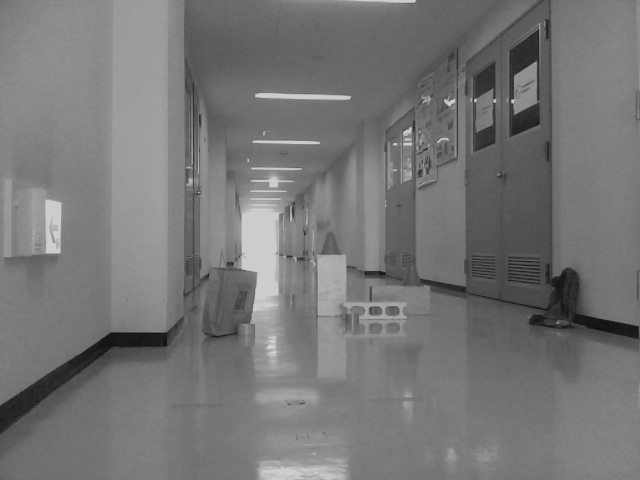
\includegraphics[width=\columnwidth]{environment.png}
\caption{Environment for collecting the data base of test images and associated positions. A collection of objects thought to be easily recognizable were scattered around to serve as landmarks.}
\label{fig:environment}
\end{figure}

In order to collect the images, a stock web camera was front-mounted to an Yamabiko robot (see Figure~\ref{fig:yamabiko}). The robot was then placed at a distance of \(2m\) from the front-most landmark, close and at a parallel angle to the right wall of the environment, and left to autonomously perform the following steps:

\begin{enumerate}
\item Turn \(60^{\circ}\) to the left;
\item Take a picture, record its position, then turn \(10^{\circ}\) to the right;
\item Repeat the previous step until collecting a total of 13 data points;
\item Turn left \(60^{\circ}\) (so it will again stand parallel to the side walls);
\item Advance \(10cm\) in a straight line;
\item Turn \(60^{\circ}\) to the {\it right};
\item Take a picture, record its position, then turn \(10^{\circ}\) to the {\it left};
\item Again, repeat the previous step until a total of 13 data points are collected;
\item Turn {\it right} \(60^{\circ}\);
\item Advance another \(10cm\);
\item Repeat the steps above until advancing a total of \(1m\);
\item Turn \(90^{\circ}\) to the left, advance \(1cm\), then turn \(90^{\circ}\) to the right;
\item Repeat steps 1-4, then move back \(1cm\);
\item Repeat steps 6-9, then move back another \(1cm\);
\item Repeat the last two steps until receding \(1m\);
\item Repeat the pattern of movement above until moving \(1m\) to the left.
\end{enumerate}

This path was designed to minimize the impact of random errors in the robot's odometer, making it so they partially cancel each other out. See Figure~\ref{fig:path} for a schematic representation. The recorded image data base amounts to 1300 images of 800 X 600 pixels in size, taken at regular intervals of \(10cm\) X \(10cm\) X \(10^{\circ}\).

\begin{figure}[h!]
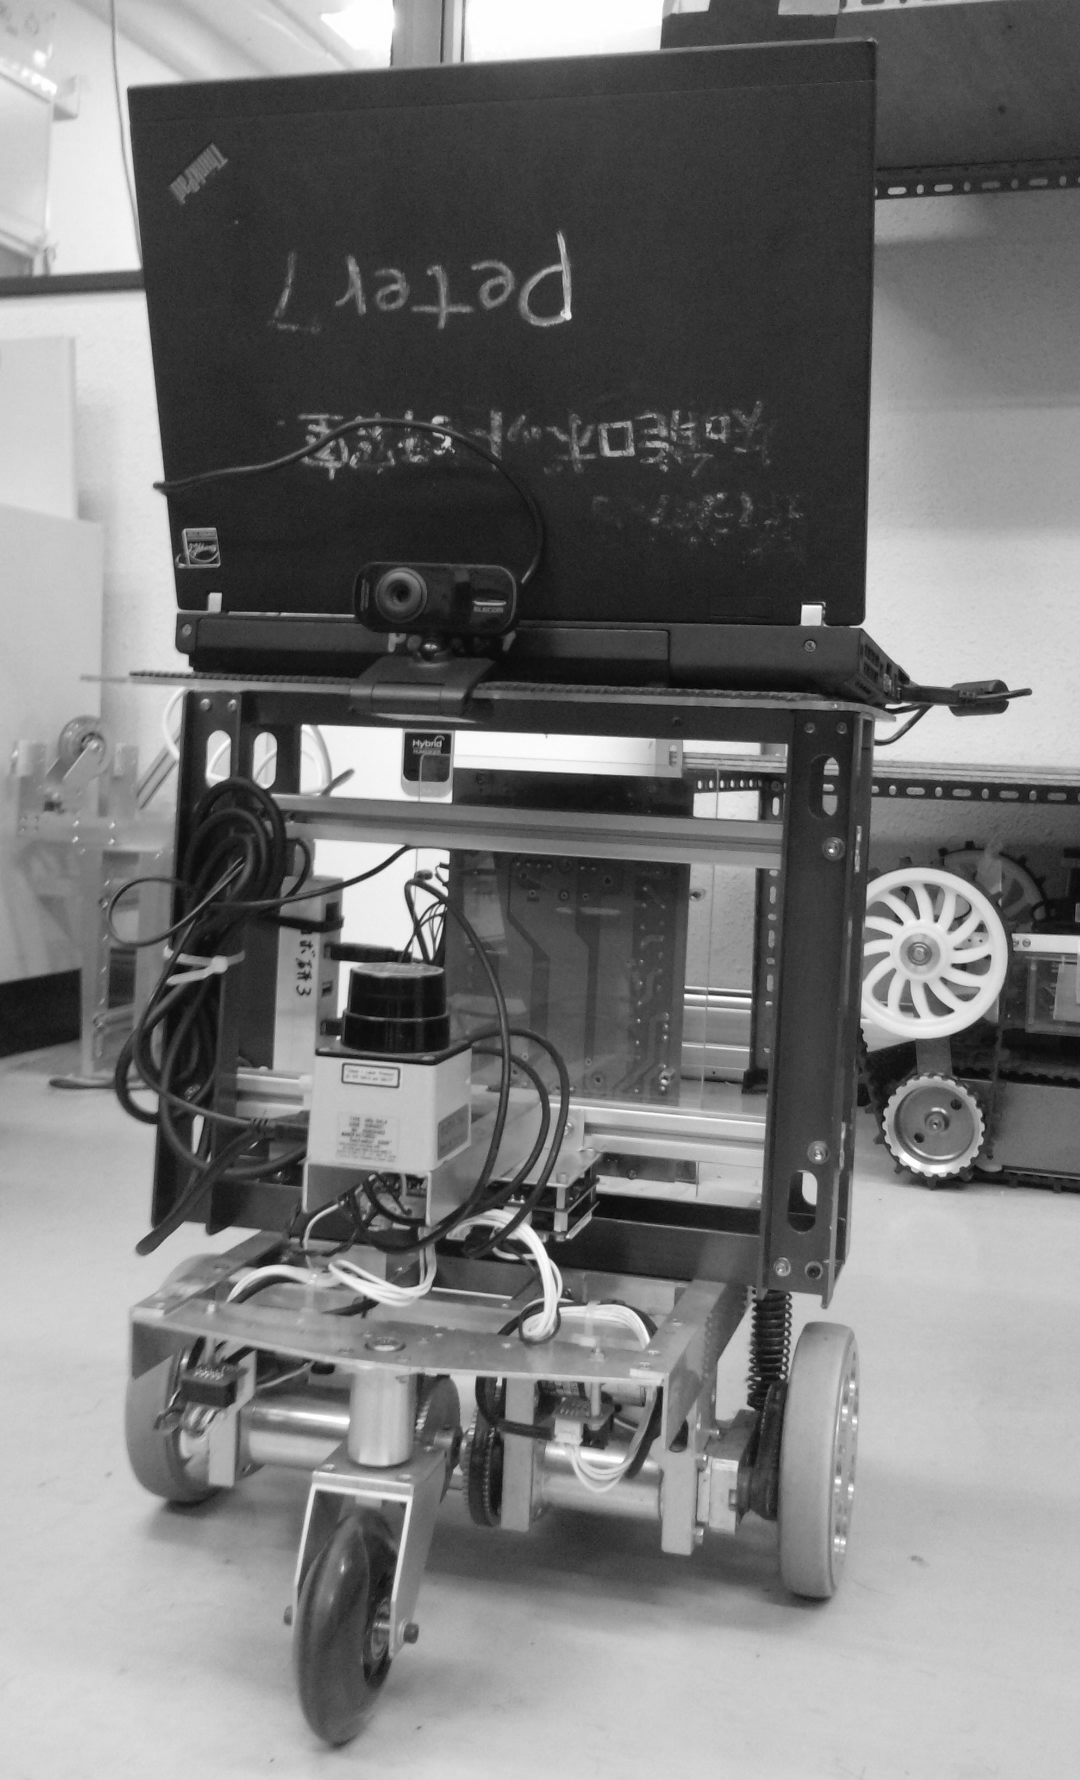
\includegraphics[width=\columnwidth]{yamabiko.png}
\caption{Yamabiko robot used to collect the database of images and positions.}
\label{fig:yamabiko}
\end{figure}

\begin{figure}[h!]
\includegraphics[width=\columnwidth]{path.pdf}
\caption{Path traveled by the Yamabiko robot throughout the test environment. At each of the 100 stops 13 pictures were taken, amounting to a total of 1300 recorded pictures.}
\label{fig:path}
\end{figure}

Pictures were named in the form {\tt still-\$i-\$j-\$k.png}, where {\tt \$i} and {\tt \$j} are respectively the forward and lateral distances (in decimeters) between the environment's origin point (at the rear-left end of the picture-taking area) and the robot's location at the time the picture was taken, and {\tt \$k} the distance between the leftmost turning point and the robot's orientation at the time (in tens of degrees). See Figure~\ref{fig:naming} for an illustration.

\begin{figure}[h!]
\includegraphics[width=\columnwidth]{naming.pdf}
\caption{Naming scheme for pictures in the test data base. Pictures at each stop are labeled with the forward and lateral distances from that stop to the origin at the rear-left, in decimeters; and also the distance from the leftmost orientation to the robot's orientation at the time, in tens of degrees.}
\label{fig:naming}
\end{figure}

\section{Landmark Extraction and Comparison}

Automatic selection of landmarks in sensory streams remains an open problem for robot navigation. Different approaches have been proposed, from employing an acquired global model of the environment to locate deviating local features, to statistical methods that attempt to maximize the utility of the extracted set, and even biological-inspired attention-based procedures. Most schemes require a learning phase before landmarks can be recognized.

For the purposes of evaluating the displacement model, a simpler strategy was devised: select the most "colorful" objects in each image as landmarks, where "colorful" is defined as the value of the Saturation channel of the HSL color space. Given an input image \(I\), the procedure is performed as follows:

\begin{enumerate}
\item Calculate \(S_I\), the HSL Saturation channel of \(I\) normalized across the range [0, 255];
\item Apply Otsu's method~\cite{otsu79} to \(S_I\), creating the binary image \(B_I\);
\item Apply an edge detection filter to \(S_I\), creating the binary edge map \(E_I\);
\item Calculate the edge-subtracted binary image \(G_I = B_I - E_I\);
\item Apply a morphological erosion operation to \(G_I\), producing the foreground mask \(F_I\);
\item Apply a morphological dilation operation to \(F_I\) followed by the inversion of all bit values, producing the background mask \(R_I\);
\item Combine background and foreground masks in a gray-scale mask \(M_I = 255 * F_I + 64 * R_I\);
\item Perform marker-based watershed segmentation of \(I\) by \(M_I\), producing the segment map \(P_I\);
\item Apply border-following segmentation to \(P_I\), extracting the list \(C_I\) of landmark contours;
\item Copy the pixels from \(I\) within each contour in \(C_I\) to new images, producing the list of landmark images \(L_I\).
\end{enumerate}

Figure~\ref{fig:segmentation} illustrates the procedure. While it is certainly not without its misses, empirical tests with the data set presented in the previous section showed the procedure can identify a sufficient number of landmarks with high consistency, successfully recovering its outlines at different distances and camera orientations.

\begin{figure}[h!]
\includegraphics[width=\columnwidth]{segmentation.pdf}
\caption{Landmark extraction procedure. (a) The input image \(I\). (b) \(S_I\), the HSL Saturation channel normalized across the range [0, 255]. (c) \(B_I\), result of applying Otsu's method to \(S_I\). (d) \(E_I\), edge map of \(S_I\). (e) Edge-subtracted binary image \(G_I = B_I - E_I\). (f) \(F_I\), morphologically-eroded version of \(G_I\). (g) \(R_I\), morphologically-dilated, inverted version of \(G_I\). (h) Gray-scale mask \(M_I = 255 * F_I + 64 * R_I\). (i) Binary segment map \(P_I\). (j) Landmark contours extracted from \(C_I\). (k) Landmark images extracted from \(I\) through the contours in \(C_I\).}
\label{fig:segmentation}
\end{figure}

A procedure for measuring landmark similarity is also required, so that different object images recovered from distinct pictures can be recognized as pertaining to the same landmark. Again a simple procedure was devised, containing the following steps:

\begin{enumerate}
\item Scale both images to dimensions equal to the average width and height between them;
\item For each of the (R, G, B) color channels plus the HSL Lightness channel, take the sum of the absolute pixel-wise difference between the scaled images;
\item Sum the channel-wise differences and divide by the scaled area.
\end{enumerate}

Figure~\ref{fig:comparison} illustrates the procedure.

\begin{figure}[h!]
\includegraphics[width=\columnwidth]{comparison.pdf}
\caption{Procedure for comparing landmark sightings. Two landmark images (a) are scaled to the average dimensions between them (b) and decomposed across Red, Blue, Green and Lightness channels (c). The sum of the pixel-wise absolute difference is computed for each channel pair (d), and channel-wise results are added up and divided by the scaled area (e).}
\label{fig:comparison}
\end{figure}

One last problem remains: given two scenes \(s_a = \{s_{a,1}, s_{a,2}, \dotsc, s_{a,m}\}\) and \(s_b = \{s_{b,1}, s_{b,2}, \dotsc, s_{b,n}\}\) with possibly \(m \neq n\), how to pair up the sightings in \(s_a\) and \(s_b\) that correspond to the same landmarks, and how to find which (if any) sightings in one scene have no pair in the other? Just selecting the pairs with highest similarity could cause one landmark from \(s_a\) to be paired with several landmarks from \(s_b\) or vice-versa -- an obvious physical impossibility, as landmarks cannot be at two places at the same time.

The chosen solution was to construct an \(m X n\) matrix \(S_{a,b}\) of pair-wise similarity measurements between \(s_a\) and \(s_b\), then apply the Kuhn–Munkres assignment algorithm to the matrix. In order to avoid pairings displaying incongruent changes (e.g. size reduction in straight forward motion, or rightward movement after a turn to the right) to be selected by the algorithm, any such cases are assigned the worst similarity value allowed by the computing environment, and discarded if nevertheless they get selected. The remaining set is used to compute the difference \(d_{a,b}\) between the two scenes. Figure~\ref{fig:assignment} illustrates the process.

\begin{figure}[h!]
\includegraphics[width=\columnwidth]{assignment.pdf}
\caption{Pairing landmark sightings between two scenes. (a) An \(m X n\) matrix of pair-wise similarity measurements is constructed. (b) If \(m > n\), additional columns are added, all filled with the highest possible measurement value \(\Lambda\) (if \(m < n\), the matrix must first be transposed, then complemented in the same manner). (c) The Kuhn–Munkres assignment algorithm returns a matrix of pairings; any selected pairings that were assigned the \(\Lambda\) value prior to running the algorithm are disregarded. (d) A list of pairings is assembled for computation of the difference between the two scenes.}
\label{fig:assignment}
\end{figure}

\section{Statistical Analysis}

If there is any truth to the monocular displacement estimation hypothesis, then differences between scenes must fulfill the following requirements:

\begin{enumerate}
\item Movement by different modes (e.g. straight v. sideways) must produce distinguishable variation patterns in change attributes;
\item Movement by different {\it amounts} on the same mode (e.g. straight \(10cm\) v. \(20cm\)) must produce variations in change attributes of similar patterns but different intensities.
\end{enumerate}

In other words, in the very least it must be possible, by analyzing the differences between two scenes separated by a limited amount of single-mode movement, to identify what was the mode of movement, and estimate its amount. This can be verified by systematically comparing all pictures in the test data base, plotting their differences so as to allow quantitative comparison of movements falling in the conditions above. Some considerations on how to split and plot the data are in order, however.

Each change has four attributes (width, height, horizontal position and vertical position) which are expected to vary distinctly across differences; it's only logical, then, that a separate plot be drawn for each attribute. Moreover, the initial picture position of a landmark sighting may influence how different movements will affect future sightings -- e.g. for straight forward movements, landmarks at the left and right sides tend to drift towards the respective borders, while those at the center only drift down -- therefore it makes sense to split results across nine vertical {\it origin bands}. Figure~\ref{fig:bands} illustrates this concept.

\begin{figure}[h!]
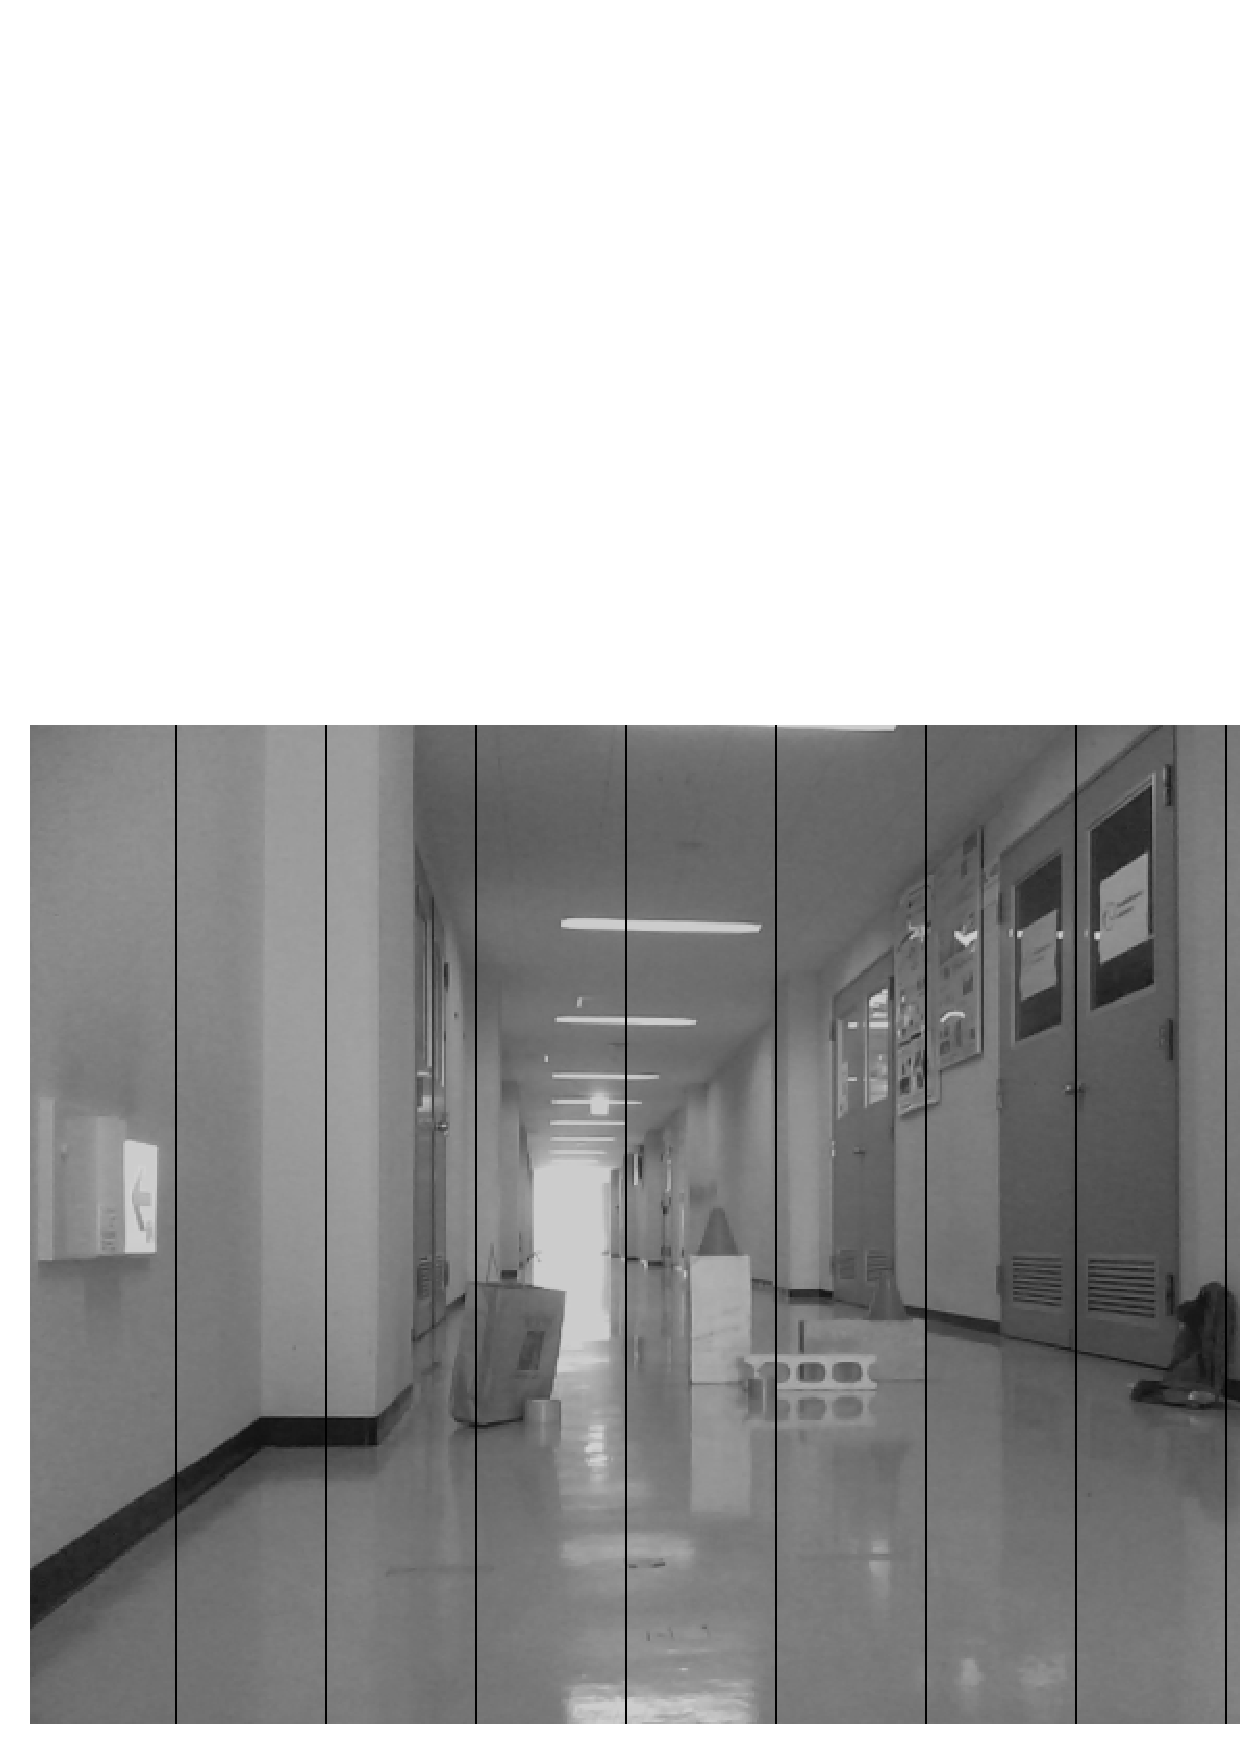
\includegraphics[width=\columnwidth]{bands.pdf}
\caption{The nine {\it origin bands} across which statistical results are split. Each band corresponds to a plot of the differences between sightings found at that band and their matches in another picture.}
\label{fig:bands}
\end{figure}

Obviously, for each movement mode, separate difference sets must be computed. Not all possible picture pairs need be compared for each mode -- only those taken at locations that can be traversed on that mode alone. Moreover, results will clearly be symmetrical between directions (e.g. straight forward and backward directions will show the same results with inverted signs), so only one direction needs to be reported for each mode. Results can then be grouped by the pair-wise distance and averaged, allowing band-wise results to be presented in a two-dimensional plot (distance X average change) instead of three-dimensional (distance X change instance X change value). Care must be taken, however, that as distance between locations increase, the number of valid image pairs differing by that amount decreases, and so statistics become less reliable. Figure~\ref{fig:distances} illustrates the problem.

\begin{figure}[h!]
\includegraphics[width=\columnwidth]{distances.pdf}
\caption{Progressive depletion of test cases with distance. On column \(0\) of the data base, if only frontward orientation is considered, there are nine image pairs traversable by straight movement alone with a distance of \(10cm\) (i.e. the pairs (0, 1), (1, 2), (2, 3), (3, 4), (4, 5), (5, 6), (6, 7), (7, 8) and , (8, 9)), but only one (the pair (0, 9)) with a distance of \(90cm\).}
\label{fig:distances}
\end{figure}

Figure~\ref{fig:straight_absolute} shows the result plots for absolute differences between straight forward movements, constructed in the manner discussed above. For each of the four change attributes -- width, height, horizontal position (U) and vertical position (V) -- a set of nine plots was drawn, corresponding to the nine origin bands in the field of view (each band is identified by the horizontal position range of sightings that fall within it).

In each plot, the horizontal axis corresponds to the distance between pairs of pictures (in decimeters). Two curves are present at each plot: the first one (drawn in black), measured by the vertical scale on the left, shows the average change for each given distance (in pixels). The second (drawn in gray), measured by the scale on the right, shows how many sighting pairs were found at each given distance. This is an important information to add perspective to the results, since (as was noted before) as the number of available samples decrease, results become less reliable.

\begin{figure}[h!]
\includegraphics[width=\columnwidth]{straight_absolute.pdf}
\caption{Result plots for absolute differences between straight forward movements. For each of the four change attributes -- width, height, horizontal position (U) and vertical position (V) -- a set of nine plots is shown, corresponding to the nine origin bands in the field of view. Each band plot is identified by the horizontal position range of sightings that fall within it. In each plot, the horizontal axis corresponds to the distance between pairs of pictures (in decimeters). Two curves are present at each plot: the first one (drawn in black), measured by the vertical scale on the left, shows the average change for each given distance (in pixels). The second (drawn in gray), measured by the scale on the right, shows how many sighting pairs were found at each given distance.}
\label{fig:straight_absolute}
\end{figure}

Looking at the plots, it's visible that for most bands, width and height increase steadily as the distance between locations increase. Also, as landmarks get close to the borders, the chance they won't be seen after the next forward movement quickly increases -- so it's no surprise that results at the outer borders tend to be more erratic.

For the horizontal position (U) plot, sightings from right-side bands tend to change rightward, while left-side band sightings largely change leftward, and sightings at the central band display very little horizontal movement. The vertical position plot (V), in contrast, only shows upward movement on average -- likely an artifact of the way samples are split across vertical bands, causing downward movement instances to be offset by upward ones.

Figure~\ref{fig:sideways_absolute} shows the result plots for absolute differences between sideways rightward movements, structured exactly like the ones for straight forward movements. In this case most bands show negligible change in width, height and vertical position, while horizontal position decreases steadily as sightings shift towards the left border.

\begin{figure}[h!]
\includegraphics[width=\columnwidth]{sideways_absolute.pdf}
\caption{Result plots for absolute differences between sideways rightward movements. For each of the four change attributes -- width, height, horizontal position (U) and vertical position (V) -- a set of nine plots is shown, corresponding to the nine origin bands in the field of view. Each band plot is identified by the horizontal position range of sightings that fall within it. In each plot, the horizontal axis corresponds to the distance between pairs of pictures (in decimeters). Two curves are present at each plot: the first one (drawn in black), measured by the vertical scale on the left, shows the average change for each given distance (in pixels). The second (drawn in gray), measured by the scale on the right, shows how many sighting pairs were found at each given distance.}
\label{fig:sideways_absolute}
\end{figure}

Figure~\ref{fig:turning_absolute} shows the result plots for absolute differences between turning rightward movements. This set differs from the previous ones in that the horizontal axis of the plots measures distances in tens of degrees instead of decimeters, but otherwise the structure is the same. It also display very similar results to the sideways case, with marked horizontal distance decreases between movements whereas other properties change little or too erratically to be considered.

\begin{figure}[h!]
\includegraphics[width=\columnwidth]{turning_absolute.pdf}
\caption{Result plots for absolute differences between turning rightward movements. For each of the four change attributes -- width, height, horizontal position (U) and vertical position (V) -- a set of nine plots is shown, corresponding to the nine origin bands in the field of view. Each band plot is identified by the horizontal position range of sightings that fall within it. In each plot, the horizontal axis corresponds to the distance between pairs of pictures (in tens of degrees). Two curves are present at each plot: the first one (drawn in black), measured by the vertical scale on the left, shows the average change for each given distance (in pixels). The second (drawn in gray), measured by the scale on the right, shows how many sighting pairs were found at each given distance.}
\label{fig:turning_absolute}
\end{figure}

Looking at the results above, it seems reasonable that straight movements could be estimated by changes in size and horizontal position of sightings, while turning and sideways movements could be estimated by horizontal position changes alone. The fact that the width and height of sightings hardly change between turning and sideways movements could also be used to distinguish them from straight movements. But to distinguish between sideways and turning movement, absolute differences alone don't seem to be enough. It is required, therefore, to look into relative difference plots to tell them apart.

Figure~\ref{fig:turning_relative} shows the result plots for relative differences between turning rightward movements, and Figure~\ref{fig:sideways_relative}, for relative differences between sideways rightward movements. In contrast to absolute plots, these are not split by bands: since the very principle of relative plots is that sightings at different image regions (and hence, bands) are compared to each other, it would make little sense to enforce this division. Otherwise their structure and measurement scales are the same as those used for absolute difference plots.

\begin{figure}[h!]
\includegraphics[width=\columnwidth]{turning_absolute.pdf}
\caption{Result plots for relative differences between turning rightward movements. For each of the four change attributes -- width, height, horizontal position (U) and vertical position (V) -- a single plot is shown. In each plot, the horizontal axis corresponds to the distance between pairs of pictures (in tens of degrees). Two curves are present at each plot: the first one (drawn in black), measured by the vertical scale on the left, shows the average change for each given distance (in pixels). The second (drawn in gray), measured by the scale on the right, shows how many sighting pairs were found at each given distance.}
\label{fig:turning_absolute}
\end{figure}

Comparing those plots, we can see that the relative change in horizontal positions increases steeply for turning movements (that is, until the depletion of test cases causes it to reverse course), whereas for sideways movements it alternates between increasing and decreasing cycles. This is in agreement with earlier observations on sighting changes for these two movement modes, and allows them to be told apart.

\section{Conclusion}

As a robot with a front-mounted camera wanders around an environment with recognizable stationary objects (or {\it landmarks}), their pictured images change in predictable ways. The {\it monocular displacement estimation hypothesis} proposes that those changes can be exploited as cues to estimate the direction and extent of physical displacement of the robot between successive camera takes.

Initial tests point towards a confirmation of the monocular displacement estimation hypothesis -- i.e. it might in fact be possible to estimate a robot's physical displacement by analyzing apparent changes in position and size of landmarks captured by a front-mounted monocular camera. All single-mode movements correlate particularly well with horizontal position changes on average; straight movements, additionally, also correlate well to changes in width and height, which are negligible in the other modes. This fact makes it possible to tell straight movements apart; but telling apart turning and sideways movements requires that relative differences to horizontal position changes be also used.

One problem that was not taken into consideration is how to make sense of mixed-mode movements, i.e. those that combine straight, turning and / or sideways movements. In this case the problem is not determining what movement mode was employed, but to what extent (if any) each mode contributed to the movement. Further tests will be required to determine the effects of different mode mixes to change attributes, and consequently how to estimate physical movements from such changes.

The evaluation of supervised learning techniques as a way to construct an approximation of \(\Psi\) also arises as a logical next step. Preliminary experiments with VG-RAM networks have shown promise in modeling the effects of mixed-mode movements to sighting changes, however estimation accuracy is limited, particularly at longer distances. The employment of more sophisticated landmark selection techniques and recording of a larger, more varied image data base will undoubtedly play an important role in such developments.

\footnotesize

\bibliographystyle{IEEEtran}
\bibliography{references}

\normalsize

\end{document}
